\bookchapter{פרק 42: התמונה המלאה של המודלים הגדולים ועבודה מעשית עם API}

\chapterintro{הפרקים הקודמים עסקו ב“איך משתפים פעולה עם AI”; הפרק הזה פותר שאלה בסיסית יותר: “איזה AI משתמשים? ואיך?”. נוף המודלים הגדולים באוגוסט 2026 עשיר במיוחד — בזירה הבינלאומית מתחרים שלושת הענקים GPT, Claude ו-Gemini, ובסין שגשגים DeepSeek, Qwen (Tongyi Qianwen), GLM, Kimi ו-Doubao. לכל מודל יש אופי ונקודות חוזקה משלו: בחירה נכונה מכפילה את התפוקה, בחירה שגויה מכפילה את המאמץ. הפרק הזה לא רק מכיר לכם את המודלים, אלא גם מלמד לחבר אותם לאפליקציות שלכם דרך API, ולבחור לפי הצרכים שלכם את תוכנית ה-Token המתאימה (חבילת שימוש).}

\booksection{א. המודלים הגדולים המרכזיים בעולם: מפת שלוש הענקים}

בשוק המודלים הגדולים הבינלאומי באוגוסט 2026 התגבשה תמונה של שלוש ענקיות: OpenAI (סדרת GPT), Anthropic (סדרת Claude) ו-Google (סדרת Gemini). לכל אחת אופי בולט משלה — נכיר אותן אחת לאחת.

\booksubsection{סדרת OpenAI GPT-5.6: כל-יכול מאוזן בכל החזיתות}

OpenAI פתחה את גל המודלים הגדולים, וסדרת GPT נותרה עד היום המודל הנפוץ ביותר בעולם. סדרת GPT-5.6 שיצאה ביולי 2026 מאמצת אסטרטגיה של שלוש מדרגות: דגל GPT-5.6 Sol לצרכי הסקה ברמה גבוהה, המאוזנת GPT-5.6 Terra לפיתוח יומיומי, והקלילה GPT-5.6 Luna לתרחישי עומס גבוה בעלות נמוכה. שלושת המודלים חולקים חלון הקשר של 1.05 מיליון Token, ותומכים כולם בקלט תמונות, קריאת פונקציות ופלט מובנה.

\begin{center}
\begin{tabularx}{\linewidth}{|X|X|X|X|X|}
\hline
\textbf{דגם} & \textbf{מדרגה} & \textbf{קלט (למיליון Token)} & \textbf{פלט (למיליון Token)} & \textbf{חלון הקשר} \tabularnewline
\hline
GPT-5.6 Sol & הדגל להסקה & 5.00 דולר (כ-36 יואן) & 30.00 דולר (כ-217 יואן) & 1.05 מיליון Token \tabularnewline
GPT-5.6 Terra & מאוזן ליומיום & 2.50 דולר (כ-18 יואן) & 15.00 דולר (כ-109 יואן) & 1.05 מיליון Token \tabularnewline
GPT-5.6 Luna & קליל בעלות נמוכה & 1.00 דולר (כ-7 יואן) & 6.00 דולר (כ-44 יואן) & 1.05 מיליון Token \tabularnewline
\hline
\end{tabularx}
\end{center}

\begin{center}\small\color{gray}תמחור סדרת OpenAI GPT-5.6 (אוגוסט 2026)\end{center}

יתרון הליבה של סדרת GPT הוא “האיזון” — הסקה, תכנות, כתיבה ורב-מודאליות, בלי נקודת תורפה בולטת. יחד עם אקוסיסטם התוספים העצום של OpenAI וקהילת המפתחים שלה, התיעוד ושרשרת הכלים הם המפותחים ביותר. לתרחישים של “לא יודעים מה לבחור”, GPT הוא התשובה הברירת-מחדל שאי אפשר לטעות בה. אבל נקודת התורפה שלו: הגישה מסין דורשת רשת מיוחדת, הביטוי בסינית מדי פעם נושא “מבטא תרגומי”, ומחירי ה-API נמצאים ברמה בינונית-גבוהה.

\textbf{חדשות טובות}\par

באוגוסט 2026 הודיעה OpenAI שהמודל המוגדר כברירת מחדל למשתמשים בחינם שודרג ל-GPT-5.6 Luna, ונפתח צ'אט טקסט ללא הגבלת כמות. משמעות הדבר: אפשר לחוות את יכולות הבסיס של GPT בעלות אפס, ולשלם רק כשנדרשת הסקה חזקה יותר או קריאות API.

\booksubsection{סדרת Anthropic Claude: התקרה של התכנות והדיוק}

אם GPT הוא הכל-יכול, הרי Claude הוא “התקרה” של עולם התכנות. סדרת Claude של Anthropic מובילה זה זמן ארוך בפער ניכר ב-SWE-bench (מבחן הבנצ'מרק להנדסת תוכנה), עם איכות חוללת קוד ויכולת הוצאה לפועל של פרויקטים ברמה הנדסית — הראשונה בתעשייה. יתרה מזאת, שיעור ההזיות של Claude (הסיכוי לייצר מידע שקרי) הוא הנמוך ביותר ברשת — כ-1\% בלבד — מה שהופך אותו מתאים במיוחד לתרחישי דיוק גבוהים כמו אקדמיה ומשפטים.

קלף המר הנוסף של Claude הוא ההקשר הענק: חלון הקשר של מיליון Token, שמאפשר “לקרוא” במכה אחת חוזים של מאות עמודים או מאגר קוד שלם בלי לפספס פרטים. בתרחישים כמו שכתוב קוד וניתוח מסמכים ארוכים זה כמעט בלתי ניתן להחלפה. Claude Code, כלי התכנות בעזרת AI לטרמינל, הגיע עד אמצע 2026 להכנסה שנתית מואצת של 2.5 מיליארד דולר — ההוכחה המובהקת ביותר להכרה ביכולת התכנות של Claude.

\begin{center}
\begin{tabularx}{\linewidth}{|X|X|X|X|X|}
\hline
\textbf{דגם} & \textbf{מדרגה} & \textbf{קלט (למיליון Token)} & \textbf{פלט (למיליון Token)} & \textbf{חלון הקשר} \tabularnewline
\hline
Claude Fable 5 & דגם הדגל & 10.00 דולר (כ-72 יואן) & 50.00 דולר (כ-362 יואן) & 1 מיליון Token \tabularnewline
Claude Opus 4.8 & דגם מקצועי & 5.00 דולר (כ-36 יואן) & 25.00 דולר (כ-181 יואן) & 1 מיליון Token \tabularnewline
Claude Sonnet 5 & דגם חסכוני & 2.00 דולר (כ-14 יואן) & 10.00 דולר (כ-72 יואן) & 1 מיליון Token \tabularnewline
\hline
\end{tabularx}
\end{center}

\begin{center}\small\color{gray}תמחור סדרת Anthropic Claude (אוגוסט 2026; ל-Sonnet 5 מוצג מחיר מבצע)\end{center}

נקודת התורפה של Claude היא המחיר — לפלט של Fable 5 יש את המחיר הגבוה ביותר מבין כל המודלים: 50 דולר למיליון Token. גם היכולות הרב-מודאליות (הבנת תמונות ווידאו) בינוניות יחסית. למפתחים עצמאיים בתקציב מוגבל, Sonnet 5 בתקופת המבצע מציע תמורה בולטת במיוחד.

\booksubsection{סדרת Google Gemini: מלך הרב-מודאליות}

סדרת Gemini של Google הגיעה ב-2026 לגרסה 3.1 Pro. הקלף המר הגדול של Gemini הוא רב-מודאליות מקורית — ניתוח תמונות וטקסט מדויק, זיהוי טבלאות ב-OCR ללא שגיאות, חילוץ פריימים מווידאו ביעילות, ותמיכה גם בניתוח עמוק של אודיו ווידאו. הוא שזור עמוקות באקוסיסטם של Google (חיפוש, דואר, שירותי ענן), ובולט באחזור מידע בזמן אמת ובהבנה חוצת מודאליות. Gemini תומך גם בקלט הקשר ענק של 2 מיליון Token — חלון ההקשר הגדול ביותר בשוק כיום.

המיקום של Gemini הוא “הבחירה הראשונה להסקה מדעית ולתרחישים רב-מודאליים”. אם הפרויקט שלכם כולל ניתוח תמונות בהיקף גדול, הבנת וידאו או חישובים מדעיים — כמעט ואין ל-Gemini מתחרה. אבל בחוללת קוד טקסט טהור הוא נופל מעט מ-Claude, והביטוי בסינית פחות טבעי מהמודלים המקומיים.

\begin{center}
\begin{tabularx}{\linewidth}{|X|X|X|X|}
\hline
\textbf{פריט השוואה} & \textbf{GPT-5.6} & \textbf{Claude Fable 5} & \textbf{Gemini 3.1 Pro} \tabularnewline
\hline
ציון כולל & 94.8 & 95.0 & 92.1 \tabularnewline
יכולת תכנות (SWE-bench) & 74.9\% & 64.3\% (Pro) & בינוני \tabularnewline
חלון הקשר & 1.05 מיליון Token & 1 מיליון Token & 2 מיליון Token \tabularnewline
יכולות מולטימודליות & מאוזנת & חלשה יחסית & החזקה ביותר \tabularnewline
שיעור הזיות & נמוך יחסית & הנמוך ביותר (כ-1\%) & נמוך יחסית \tabularnewline
זמינות בסין & דורש רשת מיוחדת & דורש רשת מיוחדת & דורש רשת מיוחדת \tabularnewline
אקוסיסטם API & המפותח ביותר & בשלבי צמיחה & קשור לאקוסיסטם של Google \tabularnewline
\hline
\end{tabularx}
\end{center}

\begin{center}\small\color{gray}השוואה בין שלושת המודלים הבינלאומיים הגדולים (אוגוסט 2026)\end{center}

\begin{tcbwarn}{שימו לב: המכשולים המעשיים לשימוש בסין}
עבור מפתחים בסין, המכשול המרכזי בשימוש ב-GPT, Claude ו-Gemini הוא הגישה לרשת. אמנם אפשר להשתמש בהם בעקיפין דרך פרוקסי של Azure, פלטפורמות אגרגציה של API ודרכים דומות, אבל את היציבות וההתאמה לתקנות צריך להעריך בעצמכם. אם הפרויקט שלכם מציב דרישות מחמירות לאבטחת מידע, מומלץ לתת עדיפות קודם למודלים הסיניים.

\end{tcbwarn}

\booksection{ב. המודלים הגדולים המרכזיים בסין: פריחה מגוונת}

ב-2026 המודלים הגדולים הסיניים כבר עברו מתפקיד ה“רודפים” לתפקיד “רצים לצד”, ובתחומים מסוימים אף הגיעו ל“הובלה”. בניגוד למחלוקת ה“מעטפות” של 2023, דגמי הדגל הסיניים של 2026 כבר שווים בהישגיהם למודלים הבינלאומיים הבכירים בהיסק לוגי, ביצירת קוד ובהבנת סינית, והפער הצטמצם לפחות מ-5\%. חשוב מכך: למודלים הסיניים יתרון בלתי נפרד בתרחישים בשפה הסינית, בעלות ובפריסה תואמת רגולציה.

\booksubsection{DeepSeek V4: מלך יחס העלות-תועלת}

חברת DeepSeek היא תופעה יוצאת דופן בקרב המודלים הגדולים הסיניים. בתחילת 2025 זעזעה DeepSeek-V3 את השוק עם המיצוב של “זולה פי עשרה מ-GPT וברמת יכולת דומה”, ובתעשייה כינו אותה “קו ההכרעה של מודלי ה-AI הכלליים” — מה שזול ממנה לא שווה לה באיכות, ומה שיקר ממנה לא מציע נפח ושפע כמוה. עד אוגוסט 2026 יצאה הגרסה הרשמית של DeepSeek V4-Pro: ארכיטקטורת MoE עם 1.6 טריליון פרמטרים, כ-49B מופעלים, תמיכה במיליון Token של הקשר ללא אובדן — ויחס העלות-תועלת שלה בקוד נחשב בעיני רבים לשיא העולמי.

DeepSeek V4 עשתה קפיצת מדרגה גדולה ביכולות ה-Agent — הציון במדד DeepSWE קפץ מ-12.8 ל-62.7 (+390\%), ו-NL2Repo עלה מ-38.5 ל-61.5. ה-API קיבל תמיכה בשני פרוטוקולים, Responses API ו-API של Anthropic, וכבר תואם לכלי תכנות מובילים כמו Codex ו-Claude Code. המשמעות: אפשר להחליף את ה-API של Claude ב-API של DeepSeek ולהשתמש בו בתוך Claude Code — העלות יורדת פי כמה, והחוויה כמעט זהה.

\begin{center}
\begin{tabularx}{\linewidth}{|X|X|X|X|X|}
\hline
\textbf{דגם} & \textbf{מיצוב} & \textbf{קלט (למיליון Token)} & \textbf{פלט (למיליון Token)} & \textbf{חלון הקשר} \tabularnewline
\hline
DeepSeek V4 Pro & היסק ברמת דגל & 3 יואן (כ-US\$0.43) & 6 יואן (כ-US\$0.87) & 1 מיליון Token \tabularnewline
DeepSeek V4 Flash & קל ומהיר & 1 יואן (כ-US\$0.14) & 2 יואן (כ-US\$0.28) & 1 מיליון Token \tabularnewline
\hline
\end{tabularx}
\end{center}

\begin{center}\small\color{gray}תמחור סדרת DeepSeek V4 (אוגוסט 2026, מחירי מבצע)\end{center}

השוואת מחירים: על אותם מיליון Token קלט + מיליון Token פלט, DeepSeek V4 Flash עולה כ-0.42 דולר, GPT-5.6 Sol עולה כ-35 דולר, ו-Claude Fable 5 עולה כ-60 דולר. פער של פי 80 עד 140.

\textbf{אזהרה ממלכודת: DeepSeek עומדת להעלות מחירים}\par

ב-6 באוגוסט 2026 הודיעה DeepSeek רשמית כי היא “מתכננת להעלות בקרוב בצורה משמעותית את התמחור של ה-API”, וייתכן שמחירי המבצע לא יימשכו זמן רב. בכלי תקשורת מסוימים דובר על העלאה אפשרית של פי 30, ונכון ל-14 באוגוסט החברה טרם פרסמה את תוכנית התמחור הסופית. בנוסף, הגרסה הרשמית של DeepSeek V4 הציגה מנגנון תמחור לפי שעות שיא ושפל — בשעות השיא מחיר הקריאה מוכפל ממש. מומלץ לעקוב אחרי ההכרזות הרשמיות לקבלת התמחור העדכני.

\booksubsection{Qwen3.7 Max (Tongyi Qianwen): הבחירה הארגונית של Alibaba Cloud}

סדרת Qwen (Tongyi Qianwen) של Alibaba Cloud נשענת על האקוסיסטם של Alibaba Cloud ומחזיקה ביתרון טבעי בפריסות ארגוניות. Qwen3.7 Max מיולי 2026 הוא דגל החברה הנוכחי: מודל Dense עם 235B פרמטרים, הקשר נייטיב של 256K שניתן להרחבה עד 1M. היתרונות המרכזיים של Qwen: אקוסיסטם קוד פתוח בשל (כל הסדרה בקוד פתוח, מ-7B ועד 235B), הבנה מדויקת של תרחישים בסינית, ואינטגרציה עמוקה עם התשתית של Alibaba Cloud.

\begin{center}
\begin{tabularx}{\linewidth}{|X|X|X|}
\hline
\textbf{דגם} & \textbf{מחיר פלט (למיליון Token)} & \textbf{תרחישי שימוש} \tabularnewline
\hline
qwen-turbo & 0.6 יואן & שאלות-תשובות פשוטות, סיווג טקסט, תעבורה גבוהה \tabularnewline
qwen-long & 2.0 יואן & עיבוד הקשר עצום של 10M \tabularnewline
qwen3.7-flash & 7.2 יואן & שיחה כללית, יצירת תוכן \tabularnewline
qwen3.7-plus & 12.0 יואן & מולטימודל (תמונות + וידאו), יצירה בסינית \tabularnewline
qwen3.7-max & 36.0 יואן & יכולת סינית ברמת דגל, משימות מורכבות \tabularnewline
\hline
\end{tabularx}
\end{center}

\begin{center}\small\color{gray}תמחור מדורג של סדרת Qwen – Tongyi Qianwen (אוגוסט 2026)\end{center}

התמחור של Qwen בנוי במדרגות — מ-qwen-turbo בעלות זעומה (0.6 יואן למיליון Token פלט) ועד דגל qwen3.7-max (36 יואן למיליון Token פלט), בכיסוי כל התרחישים — משאלות-תשובות קלות ועד היסק מורכב. לארגונים שכבר עובדים עם Alibaba Cloud, Qwen היא הבחירה הכי טבעית לשילוב.

\booksubsection{GLM-5.1 של Zhipu: המקום הראשון בסין ב-SWE-bench}

סדרת GLM של Zhipu AI בולטת מאוד ב-2026. GLM-5.1 השיגה את המקום הראשון בסין במדד SWE-bench: ארכיטקטורה היברידית MoE-Dense עם 744B פרמטרים ותמיכה במיליון Token של הקשר. מאפייניה: הבנה מדויקת של סמנטיקה סינית ותמיכה בפריסה פרטית תואמת רגולציה בסין — קריטי לתרחישי פיננסים ומגזר ציבורי שמציבים דרישות גבוהות לאבטחת מידע. התמחור של GLM-5.1: 6 יואן למיליון Token קלט ו-24 יואן למיליון Token פלט — רמת ביניים בקרב המודלים הסיניים.

\booksubsection{Kimi K3: מלך הטקסטים הארוכים במיוחד}

סדרת Kimi של Moonshot AI ידועה ביכולת לעבד טקסטים ארוכים במיוחד. Kimi K3, שיצאה ביולי 2026, מתהדרת ב-2.8 טריליון פרמטרים ונכנסה לצמרת העולמית במדדים רבים של משימות מורכבות. התרחיש המרכזי של Kimi הוא ניתוח מאגרי קוד ארוכים ואחזור מוגבר על מסמכים ארוכים — היא מסוגלת לעבד טקסט של ספר שלם או קוד של פרויקט שלם, ומצטיינת במיוחד במשימות אחזור מסוג “מחט בערימת שחת”. התמחור של Kimi גבוה יחסית (כ-12-20 יואן למיליון Token פלט), אבל בתרחישי טקסט ארוך אין לה מתחרים מבחינת יחס עלות-תועלת.

\booksubsection{Doubao: השחקן הרב-גוני של ByteDance}

סדרת Doubao של ByteDance מציגה יציבות ב-2026. Doubao Seed 2.1 Pro הוא מודל הדגל של Volcano Engine, עם 256K הקשר, ביצועים יציבים במבחנים מעשיים וחוויה בולטת בתרחישים בסינית. היתרונות של Doubao: מענק גדול של Token חינמיים כבר בהרשמה, אינטגרציה מלאה עם האקוסיסטם של Volcano Engine, ותמחור בקרב הרמות הנמוכות בסין. למתחילים שרוצים להתנסות מהר בתכנות AI, Doubao היא בחירת כניסה ללא חסמים.

\begin{center}
\begin{tabularx}{\linewidth}{|X|X|X|X|X|X|}
\hline
\textbf{פריט השוואה} & \textbf{DeepSeek V4} & \textbf{Qwen3.7 Max} & \textbf{GLM-5.1} & \textbf{Kimi K3} & \textbf{Doubao 2.1 Pro} \tabularnewline
\hline
ציון כללי & 87.5 & 89.7 & 90.5 & 88+ & 85+ \tabularnewline
יכולת תכנות & עוצמתית במיוחד & חזק & הראשון בסין ב-SWE & חזק & טובה מהממוצע \tabularnewline
הבנת סינית & מצוינת & מצוינת & מדויקת & מצוינת & מצוינת \tabularnewline
חלון הקשר & 1 מיליון & 256K-1M & 1 מיליון & ארוך במיוחד & 256K \tabularnewline
מחיר פלט (יואן למיליון) & 6 & 36 & 24 & 12-20 & 30 \tabularnewline
קוד פתוח & רישיון MIT & הסדרה כולה בקוד פתוח & קוד פתוח חלקית & קוד סגור & קוד סגור \tabularnewline
פריסה פרטית & נתמך & נתמך & נתמך & לא נתמך & לא נתמך \tabularnewline
\hline
\end{tabularx}
\end{center}

\begin{center}\small\color{gray}השוואה בין חמשת המודלים הסיניים הגדולים (אוגוסט 2026)\end{center}

מגמה חשובה אחת: תחושת “פער הדורות” בין המודלים הסיניים לבין GPT ו-Claude נעלמה. בהיסק לוגי ובתחרויות מתמטיקה, הפער בין דגלי המודלים הסיניים ל-GPT-5 עומד בדרך כלל על ספרות בודדות. בחשיבה ארכיטקטונית שיטתית ובהיסק הנדסי מורכב, Claude עדיין מוביל — הוא מציע פתרונות ארכיטקטוניים בעלי “נשמה” יותר, בעוד שהמודלים הסיניים נראים לפעמים “דוגמטיים”. אבל בתרחישים בסינית, בשליטה בעלויות ובפריסה תואמת רגולציה, למודלים הסיניים יתרון מוחץ.

\begin{center}
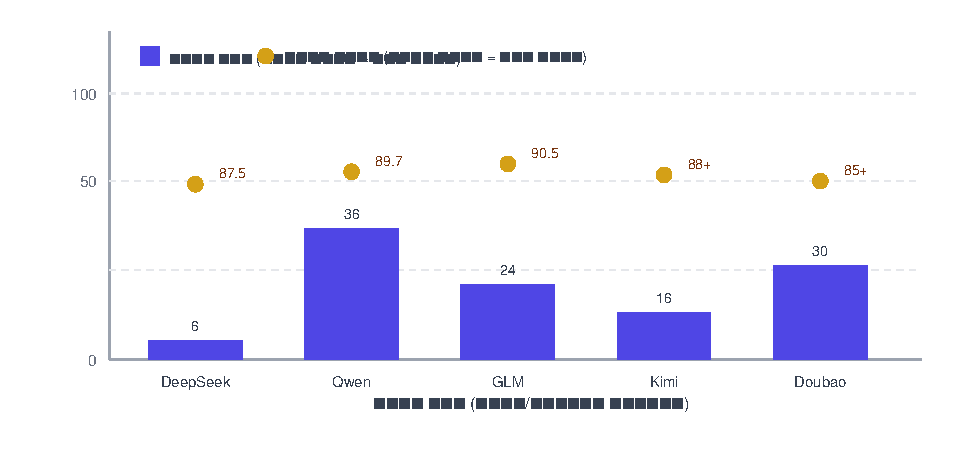
\includegraphics[width=0.92\linewidth]{figures/fig-di-si-shi-er-zhang-1}
\\[2pt]\small איור 4: השוואת מחירים וביצועים של חמשת המודלים (ככל שהמחיר נמוך יותר — טוב יותר; ככל שהציון גבוה יותר — טוב יותר)
\end{center}

\booksection{ג. מסגרת החלטות לבחירת מודל}

אחרי שהכרתם את מאפייני המודלים — איך בוחרים מודל לפרויקט שלכם? הנה לכם “שיטת ארבע השאלות” לקבלת החלטות — עונים על ארבע שאלות, ומצליחים לנעול את המודל המתאים לכם ביותר.

הפרויקט שלך נפרס בסין או בינלאומי?

בסין בחר מודלים מקומיים

|

בינלאומי אפשר לבחור מודלים זרים

המשימה המרכזית היא תכנות או משהו אחר?

תכנות Claude או DeepSeek

|

משהו אחר המשך לבחון

צריך הקשר ארוך מאוד (>500 אלף טוקנים)?

כן Gemini או Kimi

|

לא צריך המשך לבחון

התקציב דחוק?

דחוק DeepSeek או Qwen-turbo

|

לא דחוק GPT-5.6 או Claude

\begin{center}\small\color{gray}איור 5: שיטת ארבע השאלות לבחירת מודל גדול\end{center}

\begin{tcbinfo}{טיפ: אסטרטגיית שילוב}
שיטת ההחלטות הזאת איננה דוגמה — בתרחישים רבים משלבים שימוש בכמה מודלים. אסטרטגיית שילוב נפוצה: DeepSeek או Qwen לפיתוח יומיומי (עלות נמוכה, סינית טובה), Claude לעיצוב ארכיטקטוני קריטי (היסק חזק, מעט הזיות), ו-Gemini לניתוח מולטימודלי (עיבוד תמונות ווידאו). מחליפים מודל לפי הצורך, במקום “מודל אחד עד סוף החיים”.

\end{tcbinfo}

\booksection{ד. מבוא לקריאות API: חיבור למודל גדול מאפס}

הרבה מדריכי תכנות AI מלמדים רק איך להשתמש בממשק השיחה, אבל תכנות AI אמיתי — כלומר לגרום לאפליקציה שלכם לקרוא למודל גדול — מתבצע דרך API. API (Application Programming Interface, ממשק תכנות יישומים) הוא פרוטוקול תקשורת בין תוכניות. דרך ה-API, הקוד שלכם יכול לקרוא ליכולות של המודל הגדול כמו שקוראים לפונקציה.

\booksubsection{מה זה Token}

לפני שמבינים API, חייבים קודם להבין את המושג “Token”. Token הוא יחידת החיוב הבסיסית של המודלים הגדולים — אפשר לחשוב עליו כעל “יחידת הקריאה והכתיבה של ה-AI”. Token אחד מקביל בערך ל-0.75 מילים באנגלית (4 תווים), ול-0.5-1 תו סיני בסינית. קטע טקסט סיני של 1000 תווים צורך כ-1500-2000 Token.

Token אינו מספר מילים ואינו מספר תווים. המודלים הגדולים משתמשים במפרק Tokenizer ייעודי כדי לחתוך את הטקסט ל-Token. מספר ה-Token של אותה מילה עשוי להשתנות בין מודלים — למשל, המונח “בינה מלאכותית” עשוי להיות 3 Token ב-GPT ו-2 ב-DeepSeek. ה-API של רוב המודלים מחזיר את מספר ה-Token שנצרו בפועל, ואפשר לראות אותו בתשובת ה-API.

\begin{tcbinfo}{הערכה מהירה של עלות Token}
מיליון תווים בסינית שווים כ-1.5 מיליון Token. עיבוד של מיליון תווי קלט + מיליון תווי פלט עם DeepSeek V4 Flash עולה כ-0.42 דולר (כ-3 יואן); אותה כמות עם Claude Fable 5 עולה כ-60 דולר (כ-434 יואן). זו בדיוק הסיבה שבחירת המודל משפיעה ישירות על העלות של הפרויקט שלכם.

\end{tcbinfo}

\booksubsection{השגת API Key}

הצעד הראשון בשימוש ב-API של מודל גדול הוא השגת API Key — מחרוזת מפתח לאימות זהות. לכל ספק מודלים יש פלטפורמת API משלו, וצריך להירשם לחשבון וליצור API Key. לפניכם כניסות לפלטפורמות ה-API של המודלים המרכזיים ותהליך ההשגה:

\begin{center}
\begin{tabularx}{\linewidth}{|X|X|X|X|}
\hline
\textbf{מודל} & \textbf{פלטפורמת API} & \textbf{תהליך ההשגה} & \textbf{הקצבה חינמית} \tabularnewline
\hline
DeepSeek & platform.deepseek.com & הרשמה אימות זהות יצירת API Key & מענק למשתמשים חדשים \tabularnewline
Qwen (Tongyi Qianwen) & bailian.aliyun.com (פלטפורמת Bailian) & התחברות עם חשבון Alibaba Cloud הפעלת השירות יצירת Key & ניסיון חינם למשתמשים חדשים \tabularnewline
GLM (Zhipu) & open.bigmodel.cn & הרשמה אימות זהות יצירת API Key & מענק למשתמשים חדשים \tabularnewline
Kimi & platform.moonshot.cn & הרשמה אימות זהות יצירת API Key & הקצבה חינמית מוגבלת \tabularnewline
Doubao & volcengine.com (Volcano Engine) & הרשמה הפעלת Ark יצירת API Key & Token רבים במתנה עם ההרשמה \tabularnewline
OpenAI GPT & platform.openai.com & הרשמה קישור כרטיס אשראי יצירת API Key & ללא הקצבה חינמית (נדרש תשלום) \tabularnewline
Anthropic Claude & console.anthropic.com & הרשמה קישור כרטיס יצירת API Key & הקצבה קטנה למשתמשים חדשים \tabularnewline
\hline
\end{tabularx}
\end{center}

\begin{center}\small\color{gray}פלטפורמות ה-API של המודלים המרכזיים ואופן השגת ה-Key (אוגוסט 2026)\end{center}

\textbf{אזהרת אבטחה: API Key = סיסמת הארנק}\par

API Key שקול לסיסמת הארנק שלכם — כל מי שמשיג את ה-Key יכול לקרוא למודלים על חשבון ההקצבה שלכם. לכן: לעולם אל תכתבו API Key בתוך הקוד (נהלו אותו במשתני סביבה); לעולם אל תעלו למאגר Git ציבורי קוד שמכיל Key; לעולם אל תשתפו ברשתות החברתיות צילומי מסך שמציגים Key. אם ה-Key דלף — מחקו אותו מיד בפלטפורמה וצרו אחד חדש.

\booksubsection{הקריאה הראשונה ל-API}

אחרי השגת ה-API Key, אפשר לקרוא ל-API של מודל גדול בכל שפת תכנות. הנה הדגמה ב-Python של הקריאה הפשוטה ביותר — שליחת הודעה אל DeepSeek וקבלת תשובה.

\begin{lstlisting}[language=Python]
# התקנת ה-SDK: pip install openai
# DeepSeek תואם לפורמט OpenAI SDK, אפשר להשתמש ישירות
from openai import OpenAI
import os

# 1. יצירת הקליינט (מפתח ה-API נקרא ממשתנה הסביבה)
client = OpenAI(
    api_key=os.environ.get("DEEPSEEK_API_KEY"),
    base_url="https://api.deepseek.com"
)

# 2. שליחת הבקשה
response = client.chat.completions.create(
    model="deepseek-chat",  # ציון המודל
    messages=[
        {"role": "system", "content": "אתה עוזר תכנות בפייתון."},
        {"role": "user", "content": "כתוב פונקציית מיון מהיר."}
    ]
)

# 3. קבלת התשובה
print(response.choices[0].message.content)

# 4. צפייה בצריכת הטוקנים
print(f"טוקני קלט: {response.usage.prompt_tokens}")
print(f"טוקני פלט: {response.usage.completion_tokens}")
print(f"סך הטוקנים: {response.usage.total_tokens}")
\end{lstlisting}

הלוגיקה המרכזית של הקוד: יצירת קליינט (עם ה-API Key וכתובת המודל) בניית רשימת הודעות (system מגדיר את התפקיד, user הוא קלט המשתמש) שליחת הבקשה קבלת התשובה. התבנית הזאת מתאימה כמעט לכל מודל תואם OpenAI — כדי להחליף מודל מספיק להחליף את api\_key ואת base\_url. לכן מודלים סיניים רבים בוחרים בתאימות לפורמט OpenAI SDK: למפתח מספיק לשנות שתי שורות כדי להחליף מודל, ועלות המעבר זעומה.

לפניכם ההבדלים בקוד כדי לעבור למודל אחר — שימו לב, צריך לשנות רק שתי שורות:

\begin{lstlisting}[language=Python]
# DeepSeek
client = OpenAI(
    api_key=os.environ.get("DEEPSEEK_API_KEY"),
    base_url="https://api.deepseek.com"
)
# model="deepseek-chat"

# Qwen (פלטפורמת Bailian)
client = OpenAI(
    api_key=os.environ.get("DASHSCOPE_API_KEY"),
    base_url="https://dashscope.aliyuncs.com/compatible-mode/v1"
)
# model="qwen-plus"

# GLM של Zhipu
client = OpenAI(
    api_key=os.environ.get("GLM_API_KEY"),
    base_url="https://open.bigmodel.cn/api/paas/v4"
)
# model="glm-4"

# OpenAI GPT
client = OpenAI(
    api_key=os.environ.get("OPENAI_API_KEY"),
    # base_url ברירת המחדל מספיק
)
# model="gpt-5.6-terra"
\end{lstlisting}

\booksubsection{טיפול בתשובות זורמות}

ביישומים אמיתיים בדרך כלל לא כדאי לחכות שה-AI יסיים לכתוב הכול ורק אז להציג — זה מאלץ את המשתמש לחכות יותר מדי. תשובה זורמת (Streaming) מאפשרת להציג מילה אחר מילה בזמן שה-AI מייצר את התשובה, ומשפרת מאוד את חוויית המשתמש. כמו מכונת כתיבה — האותיות קופצות אחת אחרי השנייה, והתחושה של המשתמש שונה לגמרי.

\begin{lstlisting}[language=Python]
# תשובה בסטרימינג: פלט מילה אחר מילה
stream = client.chat.completions.create(
    model="deepseek-chat",
    messages=[
        {"role": "user", "content": "כתוב מדריך למיון בועות בפייתון"}
    ],
    stream=True  # הפעלת סטרימינג
)

# קבלה והדפסה בבלוקים
for chunk in stream:
    if chunk.choices[0].delta.content is not None:
        print(chunk.choices[0].delta.content, end="", flush=True)
# הפלט יופיע אות אחר אות, כמו מכונת כתיבה
\end{lstlisting}

\booksection{ה. מדריך לרכישת Token Plan}

לרוב ספקי המודלים יש שני אופני חיוב: תשלום לפי שימוש (Pay-as-you-go) ומנוי חבילה (Token Plan / Subscription). הבנת ההבדל בין שני האופנים יכולה להוזיל לכם משמעותית את עלויות השימוש.

\booksubsection{תשלום לפי שימוש מול מנוי חבילה}

\begin{center}
\begin{tabularx}{\linewidth}{|X|X|X|}
\hline
\textbf{ממד} & \textbf{תשלום לפי שימוש (Pay-as-you-go)} & \textbf{מנוי חבילה (Subscription)} \tabularnewline
\hline
אופן החיוב & משלמים לפי כמות ה-Token שנצרתה & תשלום מראש בסכום קבוע תמורת הקצבה \tabularnewline
תרחישים מתאימים & שימוש לא קבוע, קריאות מזדמנות & שימוש קבוע, קריאות בתדירות גבוהה \tabularnewline
יתרון מחיר & מחיר רגיל & זול ב-20\%-50\% מהתשלום לפי שימוש \tabularnewline
גמישות & זמין בכל עת, ללא התחייבות & דורש תשלום מראש, והקצבה עשויה לפוג \tabularnewline
טיפול בחריגה & חיוב אוטומטי לפי שימוש & מעבר לחיוב לפי שימוש לאחר גמר ההקצבה \tabularnewline
פלטפורמות מייצגות & פלטפורמות ה-API הרשמיות של כל מודל & OpenAI Plus/Pro, Claude Pro, Cursor Pro \tabularnewline
\hline
\end{tabularx}
\end{center}

\begin{center}\small\color{gray}השוואה בין שני אופני החיוב\end{center}

למתחילים מומלץ להתחיל בתשלום לפי שימוש — אין צורך בתשלום מראש, ומשלמים רק על מה שצורכים. כשהשימוש החודשי שלכם מתייצב ברמה קבועה (למשל מעל 50 יואן לחודש), שקלו לעבור למנוי חבילה כדי לקבל מחיר יחידה נמוך יותר.

\booksubsection{סקירת חבילות המנוי המרכזיות}

\begin{center}
\begin{tabularx}{\linewidth}{|X|X|X|X|}
\hline
\textbf{חבילה} & \textbf{מחיר חודשי} & \textbf{מה כלול} & \textbf{למי מתאים} \tabularnewline
\hline
ChatGPT Free & חינם & שיחות טקסט בלתי מוגבלות עם GPT-5.6 Luna & התנסות מאפס \tabularnewline
ChatGPT Plus & US\$20 לחודש & GPT-5.6 Sol, יצירת תמונות, ניתוח נתונים, גישה לתוספים & משתמשים בינוניים \tabularnewline
ChatGPT Pro & US\$200 לחודש & שימוש בלתי מוגבל בכל המודלים, גישה מוקדמת לתכונות חדשות & משתמשים מקצועיים אינטנסיביים \tabularnewline
Claude Free & חינם & מספר מוגבל של שיחות Claude & התנסות מאפס \tabularnewline
Claude Pro & US\$20 לחודש & שימוש בלתי מוגבל ב-Claude, גישה מוקדמת למודלים חדשים & מפתחים \tabularnewline
Cursor Free & חינם & מספר מוגבל של השלמות ושיחות AI & התנסות למתחילים \tabularnewline
Cursor Pro & US\$20 לחודש & השלמות AI בלתי מוגבלות, 500 בקשות מתקדמות לחודש & מפתחים יומיומיים \tabularnewline
Cursor Business & US\$40 לחודש למשתמש & עבודת צוות, ממשק ניהול, מצב פרטיות & שימוש בצוותים \tabularnewline
\hline
\end{tabularx}
\end{center}

\begin{center}\small\color{gray}חבילות מנוי לכלי AI מרכזיים (אוגוסט 2026)\end{center}

למודלים הסיניים יש תוכניות מנוי שונות במקצת. DeepSeek מחייבת בעיקר לפי שימוש ואין לה חבילת מנוי חודשית — מטעינים כסף לחשבון ומשלמים לפי השימוש בפועל. Qwen מציעה בפלטפורמת Bailian חבילות משאבים בתשלום מראש (קונים הקצבת Token מסוימת ונהנים ממחיר מוזל). גם ל-Doubao יש ב-Volcano Engine תוכניות דומות של תשלום מראש. למפתחים בסין, השילוב המשתלם ביותר הוא בדרך כלל: DeepSeek בתשלום לפי שימוש (פיתוח יומיומי) + ההקצבה החינמית של Doubao (התנסות ובדיקות).

\booksubsection{פלטפורמות אגרגציה של API}

אם אתם צריכים להשתמש בכמה מודלים במקביל, פלטפורמת אגרגציה של API היא פתרון נוח שחוסך כאב ראש. פלטפורמת אגרגציה נותנת API Key אחיד אחד, ודרכו אפשר לקרוא לעשרות מודלים ברחבי העולם — בלי להירשם בנפרד בכל פלטפורמה.

\begin{center}
\begin{tabularx}{\linewidth}{|X|X|X|X|}
\hline
\textbf{פלטפורמה} & \textbf{מאפיינים} & \textbf{יתרון מחיר} & \textbf{תרחישים מתאימים} \tabularnewline
\hline
OpenRouter (openrouter.ai) & פלטפורמת אגרגציה בינלאומית — Key אחד לקריאה למודלים מכל העולם & מחירים שקופים, השוואת מחירים בזמן אמת & למי שצריך להחליף בגמישות בין מודלים בינלאומיים \tabularnewline
SiliconFlow (siliconflow.cn) & פלטפורמת אגרגציה סינית — מציעה API למגוון מודלים סיניים & זול ב-20\%-30\% מהרשמי & מפתחים בסין, השוואת מחירים בין מודלים \tabularnewline
Azure OpenAI (פרוקסי של Microsoft) & ה-API של OpenAI בגישור של Microsoft Azure & Batch API בהנחה של 50\% & קריאות OpenAI ברמה ארגונית, משימות אסינכרוניות בהיקף גדול \tabularnewline
Baidu Qianfan (qianfan.baidubce.com) & פלטפורמת ענן ה-AI של Baidu, המציעה מודלים כמו ERNIE (Wenxin) & מענק למשתמשים חדשים & משתמשים באקוסיסטם של Baidu \tabularnewline
\hline
\end{tabularx}
\end{center}

\begin{center}\small\color{gray}פלטפורמות אגרגציה מרכזיות ל-API (אוגוסט 2026)\end{center}

\textbf{אזהרה ממלכודת: אל תקנו “Key משותף”}\par

אל תקנו “API Key משותפים” בפלטפורמות כמו Taobao או Xianyu — Key כאלה בדרך כלל ממקור לא ברור, עלולים להיחסם בכל רגע, וכרוכים גם בסיכון לדליפת מידע. השיגו API Key תמיד דרך הפלטפורמות הרשמיות או פלטפורמות אגרגציה מוכרות.

\booksubsection{אסטרטגיות לאופטימיזציה של עלויות}

בחירת המודל הנכון היא רק הצעד הראשון; גם איך “משתמשים בחוכמה” חשוב לא פחות. לפניכם כמה אסטרטגיות אופטימיזציה של עלויות שהוכחו בפועל:

\begin{enumerate}
  \item נצלו פגיעות מטמון. מודלים רבים מציעים תכונת “מטמון” — כשהבקשה שלכם כוללת תוכן שכבר עובד קודם (כמו הודעת המערכת), החלק הזה מחויב במחיר זעום. ב-DeepSeek מחיר פגיעת מטמון הוא 1/60 בלבד מהמחיר הרגיל. הציבו את הודעת המערכת הקבועה בראש רשימת ההודעות כדי למקסם פגיעות מטמון.
  \item ניתוב מדורג — מודל זול למשימות פשוטות ומודל יקר למשימות מורכבות. למשל: DeepSeek V4 Flash לסיווג טקסט (פלט ב-2 יואן למיליון Token), ו-Claude לעיצוב ארכיטקטוני (פלט ב-181 יואן למיליון Token). בפרויקט טיפוסי 80\% מהקריאות יכולות לעבוד עם המודל הזול.
  \item הגבילו את אורך הפלט. ה-API מחויב לפי Token פלט — ככל שהפלט ארוך יותר, כך הוא יקר יותר. בתרחישים שבהם אין צורך בנאומים ארוכים, הגדירו את הפרמטר max\_tokens כדי להגביל את אורך הפלט ולמנוע מה-AI “לפטפט יותר מדי”.
  \item השתמשו ב-Batch API למשימות שאינן בזמן אמת. אם יש לכם המון משימות שלא דורשות תשובה מיידית (כמו תיוג נתונים בכמויות או סיכום מסמכים), Batch API נותן הנחה של 50\%. גם OpenAI וגם Azure מציעות את התכונה הזאת.
  \item עקבו אחרי צריכת ה-Token. לרוב פלטפורמות ה-API יש לוח בקרה עם סטטיסטיקות שימוש. בדקו מעת לעת את פילוח הצריכה, מצאו את הקריאות שצורכות הכי הרבה Token ובצעו אופטימיזציה ממוקדת. התאמה קטנה של Prompt (למשל להחליף “הסבר בהרחבה” ב“הסבר ב-3 משפטים”) יכולה לחסוך 50\% מה-Token.
\end{enumerate}

\begin{center}
\begin{tabularx}{\linewidth}{|X|X|X|X|}
\hline
\textbf{אסטרטגיה} & \textbf{היקף החיסכון} & \textbf{קושי היישום} & \textbf{הסבר} \tabularnewline
\hline
פגיעות מטמון & עד 98\% & נמוך & תוכן קבוע בתחילת ההודעות \tabularnewline
ניתוב מדורג & 50\%-80\% & בינוני & מודל זול למשימות פשוטות \tabularnewline
הגבלת אורך פלט & 30\%-60\% & נמוך & הגדרת הפרמטר max\_tokens \tabularnewline
Batch API & 50\% & נמוך & עיבוד באצווה למשימות שאינן בזמן אמת \tabularnewline
אופטימיזציה של Prompt & 20\%-50\% & בינוני & לייעל את ה-Prompt ולהפחית מיותרים \tabularnewline
\hline
\end{tabularx}
\end{center}

\begin{center}\small\color{gray}אסטרטגיות אופטימיזציה של עלויות והשפעתן (אוגוסט 2026)\end{center}

\booksection{ו. התנסות מעשית: חיבור ה-API של מודל גדול בפרויקט}

נסיים את הפרק בתרגיל מעשי מלא — יצירת “מחולל סיכומים AI”: המשתמש מזין טקסט ארוך, והתוכנה קוראת ל-API של מודל גדול ליצירת סיכום. התרגיל מציג את התהליך המלא של קריאת API: הגדרת סביבה, קריאת API, טיפול בשגיאות ושליטה בעלויות.

\begin{lstlisting}[language=Python]
# ai_summarizer.py - מחולל תקצירים עם AI
import os
from openai import OpenAI

# 1. הגדרה (מפתח ה-API נקרא ממשתנה הסביבה, לעולם לא מקודד בקוד)
client = OpenAI(
    api_key=os.environ.get("DEEPSEEK_API_KEY"),
    base_url="https://api.deepseek.com"
)

def summarize(text: str, max_length: int = 200) -> dict:
    """מייצר תקציר של הטקסט

    Args:
        text: הטקסט המקורי לתקצור
        max_length: אורך מרבי לתקציר (מספר טוקנים)

    Returns:
        dict: כולל את התקציר ונתוני צריכת הטוקנים
    """
    try:
        response = client.chat.completions.create(
            model="deepseek-chat",
            messages=[
                {
                    "role": "system",
                    "content": "אתה מחולל תקצירים."
                               "סכם את הטקסט של המשתמש בשפה צלולה ותמציתית."
                               "התקציר לא עולה על 3 משפטים."
                },
                {
                    "role": "user",
                    "content": f"סכם את הטקסט הבא:\n\n{text}"
                }
            ],
            max_tokens=max_length,  # מגביל את אורך הפלט
            temperature=0.3  # טמפרטורה נמוכה = יציב יותר
        )

        return {
            "success": True,
            "summary": response.choices[0].message.content,
            "input_tokens": response.usage.prompt_tokens,
            "output_tokens": response.usage.completion_tokens,
            "total_tokens": response.usage.total_tokens
        }

    except Exception as e:
        return {
            "success": False,
            "error": str(e)
        }

# 2. דוגמת שימוש
if __name__ == "__main__":
    long_text = """
    (הדבק כאן טקסט ארוך...)
    """

    result = summarize(long_text)

    if result["success"]:
        print(f"תקציר: {result['summary']}")
        print(f"טוקנים שנצרכו: {result['total_tokens']}")
        # אומדן עלות: DeepSeek V4 Flash
        cost = result['total_tokens'] * 0.000004  # $\approx$ 0.4 סנט לכל 1000 טוקנים
        print(f"עלות משוערת: {cost:.4f} יואן")
    else:
        print(f"שגיאה: {result['error']}")
\end{lstlisting}

הקוד הזה מדגים כמה שיטות עבודה מומלצות לקריאות API: ה-API Key נקרא ממשתני סביבה ולעולם אינו מקודד ישירות בקוד; לפונקציה תיעוד ברור ורמזי טיפוסים; הוגדר max\_tokens להגבלת אורך הפלט; ה-temperature מוגדר לערך נמוך (0.3) לקבלת פלט יציב יותר; יש טיפול מלא בשגיאות; והקוד מחזיר מידע על צריכת ה-Token למעקב אחרי עלויות. כשאתם מבקשים מה-AI לכתוב את הקוד הזה, אפשר לספר לו את הדרישות האלה — הוא לגמרי מסוגל לממש אותן בשבילכם.

המסקנה הסופית של הפרק: המודלים הם "התחמושת", המתודולוגיה היא "הטקטיקה". בחירת תחמושת נכונה מקלה על הקרב, אבל בלי טקטיקה טובה גם התחמושת הטובה ביותר לא תזכה במלחמה. עכשיו אתה מכיר את המאפיינים של כל מודל ואת השימוש ב-API – ה"מחסן" שלך מלא; איך לנהל את הקרב זה תלוי במתודולוגיית החשיבה מהפרקים הקודמים.

\begin{tcbpractice}{הידיים על המקלדת: הריצו את הקריאה הראשונה שלכם ל-API}
הירשמו לפלטפורמה של מודל סיני (מומלצות DeepSeek או Zhipu — שתיהן מעניקות הקצבה למשתמשים חדשים), צרו API Key, שימו אותו במשתני הסביבה של המערכת (ולא בקוד!), ואז הריצו את קוד “הקריאה הראשונה ל-API” שלמעלה. ברגע שתראו את תשובת ה-AI מודפסת על המסך — חציתם את הקו שבין “להשתמש ב-AI” לבין “לבנות אפליקציית AI”.

\end{tcbpractice}

\begin{tcbsummary}{סיכום הפרק}
\begin{itemize}
  \item שלוש המובילות הבינלאומיות: GPT-5.6 (מאוזן ורב-יכולות), Claude (פסגת התכנות + שיעור הזיות של 1\% בלבד), Gemini (מלך המולטימודל + 2 מיליון הקשר)
  \item חמש המובילות הסיניות: DeepSeek V4 (מלך יחס העלות-תועלת, שימו לב להכרזה על העלאת מחירים), Qwen3.7 (רמה ארגונית), GLM-5.1 (הראשון בסין ב-SWE), Kimi K3 (טקסטים ארוכים במיוחד), Doubao (כניסה חינמית)
  \item שיטת ארבע השאלות: איפה מפריסים? תכנות או משהו אחר? הקשר ארוך במיוחד? רגישות לתקציב?
  \item Token היא יחידת החיוב: תו סיני אחד שווה כ-1.5-2 Token; מיליון תווים בסינית שווים כ-1.5 מיליון Token
  \item API Key = סיסמת הארנק: ניהול במשתני סביבה, לעולם לא מקודד בקוד ולא נשלח ל-Git
  \item המודלים הסיניים תואמים בדרך כלל ל-OpenAI SDK: כדי להחליף מודל משנים רק את שתי השורות api\_key ו-base\_url
  \item חמש דרכים לחסוך: פגיעות מטמון, ניתוב מדורג, הגבלת פלט, Batch API, מעקב אחרי שימוש
\end{itemize}

\end{tcbsummary}
